\documentclass{article}

\usepackage[hmargin=2cm,vmargin=2.5cm]{geometry}
\usepackage{mathtools,amssymb,amsthm,mathrsfs}
\usepackage{cite}
\usepackage{mathtools} % Allows use of equation environment
\usepackage{graphicx} % Allows you to import pictures
\usepackage{verbatim} % Allows the use of the verbatim environment (necessary printing code)
\usepackage{wrapfig} % Allows use of the wrapfig environment
\usepackage{fixltx2e} % Let's you use subscript and superscript outside of equations
\usepackage[version=3]{mhchem} % Automatic subscripting of chemical equations
\usepackage{appendix} % Allows use of appendices
\numberwithin{equation}{section} %Sets numbering style
\setlength{\parindent}{0cm} % Sets paragraph indentation to zero
\usepackage{microtype} % Used to disable ligatures, when combined with next line
%\DisableLigatures{encoding = *, family = *} % Used to disable ligatures
%\frenchspacing % Disables additional spacing after full stops
% All of the below creates the acknowledgements environment
\makeatletter
\newcommand\ackname{Acknowledgements}
\if@titlepage
\newenvironment{acknowledgements}{%
\titlepage
\null\vfil
\@beginparpenalty\@lowpenalty
\begin{center}%
\bfseries \ackname
\@endparpenalty\@M
\end{center}}%
{\par\vfil\null\endtitlepage}
\else
\newenvironment{acknowledgements}{%
\if@twocolumn
\section*{\abstractname}%
\else
\small
\begin{center}%
{\bfseries \ackname\vspace{-.5em}\vspace{\z@}}%
\end{center}%
\quotation
\fi}
{\if@twocolumn\else\endquotation\fi}
\fi
\makeatother

%\newcommand{\Pr}{\text{Pr}}


\begin{document}

\begin{center}
\textsc{\LARGE University of Sheffield}\\[1.5cm]
\textsc{\Large EPSRC Summer Project}\\[0.5cm]
{ \huge \bfseries Phase Diffusion with Evaporation Scheme in Thin Polymer Films}\\
% Author and supervisor
\begin{minipage}{0.4\textwidth}
\begin{flushleft} \large
\emph{Author:}\\
Josh Kettlewell\\
090155185
\end{flushleft}
\end{minipage}
\begin{minipage}{0.4\textwidth}
\begin{flushright} \large
\emph{Supervisor:} \\
Prof. Nigel Clarke\\
\end{flushright}
\end{minipage}
\vfill
% Bottom of the page
{\large August 2012}
\end{center}
\thispagestyle{empty}
\newpage



\thispagestyle{empty}
\begin{abstract}
The purpose of this project was to create a 3 dimensional simulation of phase diffusion occurring in a ternary system under solvent evaporation conditions. The desire was to create a video showing an ordering plane forming from which the solvent evaporation that propagates downwards as evaporation progresses. The project was based on previous work By Nigel Clarke ,Ian C. Henderson and G.A Buxton \cite{main}. 
\end{abstract}


\begin{figure}[h]
\begin{center}
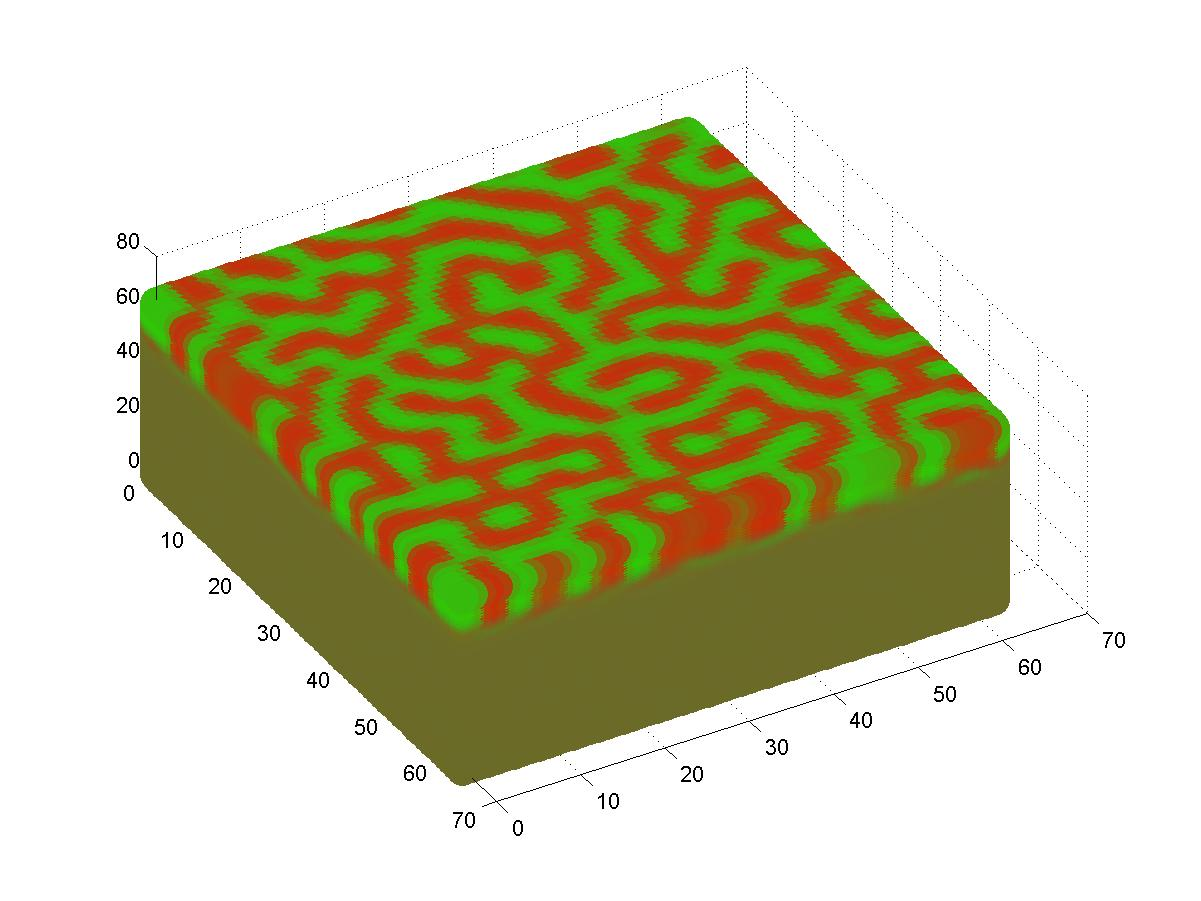
\includegraphics[width=8cm]{diffusion_3.jpg}
\label{info3}
\end{center}
\end{figure}

\begin{figure}[h]
\begin{center}
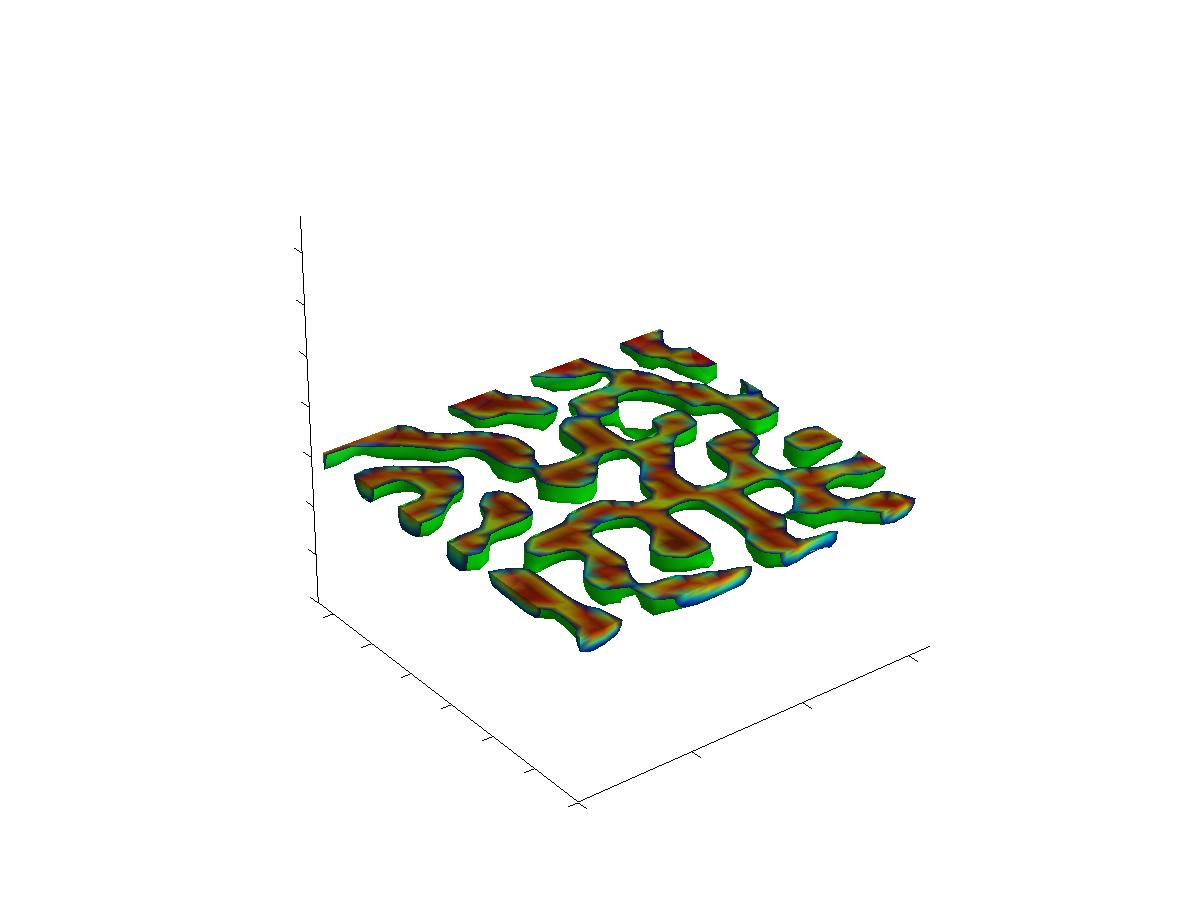
\includegraphics[width=10cm]{diffusion_5.jpg}
\label{info2}
\end{center}
\end{figure}

\newpage
\setcounter{page}{1}

\section{Program files}
\subsection{CUDA and preliminary work}
The program is written in C/C++ with the CUDA extension within the visual studio environment. The Project can simply be opened with all its competent files by opening summer\textunderscore project2 which is of a Microsoft visual studio solution filetype. The only other file which need be opened is the input file named phasesep3d which is a text document. Once summer\textunderscore project2 is opened all of the files can be viewed. There are seven files which are as follows; kernel (a .cu file), and  cudafiles1, cudafiles2, initialise\textunderscore and\textunderscore addnoise, headerfile, graphterms and getvariables (all of which are .h files). It may be immediately obvious that these header files could all be combined into a single header file, however, for clarity they have been left as separate files as each contains functions which act on different aspects of the program which makes debugging and editing the program significantly easier. Should the program wish to be used with different input variables then only the text document phasesep3d need be edited. The final version of the system, at the time of writing, is version four which differs for version 3 as height variations are taken into account by changing the delta\textunderscore z array to include a specific value for every point on the lattice.

\subparagraph{Equations} The main equations governing the system describe the rate of change of polymer concentration at each lattice point, They calculated as follows;
 
 \begin{align}
\frac{\partial \phi _{A}(x, \tau )}{\partial \tau}=\nabla \Lambda _{AA} \nabla &[\frac{\ln \phi _{A}}{N_{A}} - \frac{\ln (1- \phi _{A} - \phi _{B})}{N_{C}}+\chi _{AC}(1-2\phi _{A} - \phi _{B})+\phi _{B}(\chi _{AB} - \chi _{BC}))  \notag \\
& + \frac{1}{36}((\frac{1}{(1 - \phi _{A} - \phi _{B})^2} - \frac{1}{\phi _{A}^2})(\nabla \phi _{A})^2 +\frac{1}{(1-\phi _{A} - \phi _{B})^2}(\nabla \phi _{B})^2) \notag \\
& -(\frac{1}{18}(\frac{1}{(1- \phi _{A} - \phi _{B})} + \frac{1}{\phi _{A}})\nabla ^2\phi _{A} + \frac{1}{(1 - \phi _{A} - \phi _{B})}\nabla ^2\phi _{B})] \notag \\
+ \nabla \Lambda _{AB} \nabla &[\frac{\ln \phi _{B}}{N_{B}} - \frac{\ln (1- \phi _{A} - \phi _{B})}{N_{C}}+\chi _{BC}(1-\phi _{A} - 2\phi _{B})+\phi _{A}(\chi _{AB} - \chi _{AC}))  \notag \\
& + \frac{1}{36}((\frac{1}{(1 - \phi _{A} - \phi _{B})^2} - \frac{1}{\phi _{B}^2})(\nabla \phi _{B})^2 +\frac{1}{(1-\phi _{A} - \phi _{B})^2}(\nabla \phi _{A})^2) \notag \\
& -(\frac{1}{18}(\frac{1}{(1- \phi _{A} - \phi _{B})} + \frac{1}{\phi _{B}})\nabla ^2\phi _{B} + \frac{1}{(1 - \phi _{A} - \phi _{B})}\nabla ^2\phi _{A})] 
\end{align}

 \begin{align}
\frac{\partial \phi _{B}(x, \tau )}{\partial \tau}=\nabla \Lambda _{BA} \nabla &[\frac{\ln \phi _{A}}{N_{A}} - \frac{\ln (1- \phi _{A} - \phi _{B})}{N_{C}}+\chi _{AC}(1-2\phi _{A} - \phi _{B})+\phi _{B}(\chi _{AB} - \chi _{BC}))  \notag \\
& + \frac{1}{36}((\frac{1}{(1 - \phi _{A} - \phi _{B})^2} - \frac{1}{\phi _{A}^2})(\nabla \phi _{A})^2 +\frac{1}{(1-\phi _{A} - \phi _{B})^2}(\nabla \phi _{B})^2) \notag \\
& -(\frac{1}{18}(\frac{1}{(1- \phi _{A} - \phi _{B})} + \frac{1}{\phi _{A}})\nabla ^2\phi _{A} + \frac{1}{(1 - \phi _{A} - \phi _{B})}\nabla ^2\phi _{B})] \notag \\
+ \nabla \Lambda _{BB} \nabla &[\frac{\ln \phi _{B}}{N_{B}} - \frac{\ln (1- \phi _{A} - \phi _{B})}{N_{C}}+\chi _{BC}(1-\phi _{A} - 2\phi _{B})+\phi _{A}(\chi _{AB} - \chi _{AC}))  \notag \\
& + \frac{1}{36}((\frac{1}{(1 - \phi _{A} - \phi _{B})^2} - \frac{1}{\phi _{B}^2})(\nabla \phi _{B})^2 +\frac{1}{(1-\phi _{A} - \phi _{B})^2}(\nabla \phi _{A})^2) \notag \\
& -(\frac{1}{18}(\frac{1}{(1- \phi _{A} - \phi _{B})} + \frac{1}{\phi _{B}})\nabla ^2\phi _{B} + \frac{1}{(1 - \phi _{A} - \phi _{B})}\nabla ^2\phi _{A})] 
\end{align}

where

 \begin{align}
\Lambda _{ij} = (\partial _{ij} - \phi _{i})-\phi _{j} + 2\phi _{i} \phi _{j}.
\end{align}
These differentials are calculated for each lattice point in the system and multiplied by the time step to give $\partial \phi _{i}$ which is then added to the previous value of $\phi _{i}$ to give the current value. 


\subparagraph{How the system works}  The system uses the FDTD method to calculate the evolution of the system. Initially three 1D arrays are created (which represents the 3D system, each array being the A,B and C concentration at each point) and reads in variables from the input file "phasesep3d". The data from the input file is then used the create the specifics of the system (such the lattice spacing and the amount of solvent). The arrays are copied over to the GPU and a fraction of the solvent from the top layer. The average amount of solvent in each layer is then calculated and then used to define the spacing in the x axis between that layer and the neighbouring layers. This simulates the evaporation scheme as less solvent in the layer increases the forces between the polymers.   

\subparagraph{The importance of CUDA and parallelism} The program makes use of the highly parallel properties of the system by calculating the finite difference to each point on the lattice simultaneously. This is done by using the blocks and threads properties of the GPU to map to the system, meaning each thread represents its own lattice point. The program could be rewritten to run on a CPU using a complex series of nested loops however, it would take a vastly larger period of time. 


\section{The files} Description of functions in each file

\subsection{kernel} The kernel is the main file which calls in the other functions. It contains the main function which creates the arrays, gives percentage of a or b polymer at each grid point and begins the diffusion and evaporation simulation. The diffusion and evaporation scheme is achieved by using nested loops within which the inner loop iterates the system several times (by an input from the input file) and the outer loop copies data from the GPU to the CPU and saves it to a text file. An estimated time for completion of the simulation is calculated after the first loop and a percentage of completion is given with each loop \footnote{be aware that the estimated time can sometimes increase dramatically and if this is seen it is usual best to restart the simulation. This error is presumed to be due to hung threads.}. It is worth noting that only 2 of the arrays are handed to the GPU (the A and B arrays) and the third is calculated when the data is saved my taking the remained of these arrays from 1 (this calculation is completed in the graph terms file). 

\subsection{headerfile} This file simply contains declares variables so they need not be defined in main. Most notably is also globally defines the length of the system in the x,y, and z components. These numbers should be powers of 2. 

\subsection{cudafiles2} This file contains slightly differing functions depending on whether the third of forth version of the project is being used. In the third there are four functions; the first initialise the solvent in the system using the solvent value for the input file by reducing the values of the a and b array values by an equal percentage which is specified. The second removes the solvent from the third layer from the top \footnote{this layer represents the actual top layer due to boundary conditions}. The third  and fourth functions sum the amount of solvent in the x axis and y axis, respectively, and uses these values to set the z separation for each layer. The z value for each layer is stored as an array on the GPU and is printed to screen before the first loop to show the initial z values; these results should be equal to the initial delta x and y values. //
In version 4, the summation schemes are not present and has been replaced with files named "make deltas", which uses the amount of solvent in each cell to set specific delta values for z, and "find\textunderscore height \textunderscore z which calculates the specific height of each lattice point. 

\subsection{cudafiles1}  Here the surface boundry conditions are applied at the top and the bottom. The next function then calculates the value of mu calc from equations 1.1. and 1.2.  \begin{align}
\mu _{A1} = \mu _{B1} = &[\frac{\ln \phi _{A}}{N_{A}} - \frac{\ln (1- \phi _{A} - \phi _{B})}{N_{C}}+\chi _{AC}(1-2\phi _{A} - \phi _{B})+\phi _{B}(\chi _{AB} - \chi _{BC}))  \notag \\
& + \frac{1}{36}((\frac{1}{(1 - \phi _{A} - \phi _{B})^2} - \frac{1}{\phi _{A}^2})(\nabla \phi _{A})^2 +\frac{1}{(1-\phi _{A} - \phi _{B})^2}(\nabla \phi _{B})^2) \notag \\
& -(\frac{1}{18}(\frac{1}{(1- \phi _{A} - \phi _{B})} + \frac{1}{\phi _{A}})\nabla ^2\phi _{A} + \frac{1}{(1 - \phi _{A} - \phi _{B})}\nabla ^2\phi _{B})]
\end{align}

 \begin{align}
\mu _{A2} = \mu _{B2} = &[\frac{\ln \phi _{B}}{N_{B}} - \frac{\ln (1- \phi _{A} - \phi _{B})}{N_{C}}+\chi _{BC}(1-\phi _{A} - 2\phi _{B})+\phi _{A}(\chi _{AB} - \chi _{AC}))  \notag \\
& + \frac{1}{36}((\frac{1}{(1 - \phi _{A} - \phi _{B})^2} - \frac{1}{\phi _{B}^2})(\nabla \phi _{B})^2 +\frac{1}{(1-\phi _{A} - \phi _{B})^2}(\nabla \phi _{A})^2) \notag \\
& -(\frac{1}{18}(\frac{1}{(1- \phi _{A} - \phi _{B})} + \frac{1}{\phi _{B}})\nabla ^2\phi _{B} + \frac{1}{(1 - \phi _{A} - \phi _{B})}\nabla ^2\phi _{A})] ]
\end{align}
 where all gradients are calculated using central difference. mu\textunderscore surf then sets the boundary conditions for this array.  phi\textunderscore diff1 and phi \textunderscore diff2 then calculate the diffusion. \\
 In the fourth version of the program there is also a function names find\textunderscore z\textunderscore height which uses the delta z values to find the height of each cell. This information in then plotted in graph\textunderscore  terms. 

 \begin{align}
\frac{\partial \phi _{A}(x, \tau )}{\partial \tau} = \nabla \Lambda _{AA} \nabla \mu _{A1} + \nabla \Lambda _{AB} \nabla \mu _{A2} 
\end{align}
and
 \begin{align}
\frac{\partial \phi _{B}(x, \tau )}{\partial \tau} = \nabla \Lambda _{BA} \nabla \mu _{B1} + \nabla \Lambda _{BB} \nabla \mu _{B2} 
\end{align}

by first taking a forward difference for the gradient and then the backwards difference. These functions can not be combined into a single function as all of the blocks must calculate the values of 
 \begin{align}
\Lambda _{AA} \nabla \mu _{A1}, \notag \\
\Lambda _{AB} \nabla \mu _{A2}, \notag \\
\Lambda _{BA} \nabla \mu _{B1}, \notag \\
\Lambda _{BB} \nabla \mu _{B2}
\end{align}
for its current lattice point before it can continue. These values are all stored on arrays on the GPU. The advantage of using this method is that each lattice point is not only taking into account its 6 nearest neighbours, but also the 6 neighbours of its six nearest neighbours. This was noticed when the method was first implemented as it resulted in a much smoother phase diffusion process.  

\subsection{initialise and addnoise} Initialise fills the arrays of phi\textunderscore A and phi\textunderscore B with values using the value of phi\textunderscore bar from the input file. The value of phi\textunderscore A and phi\textunderscore B at each point add to 1 but may not necessarily be equal depending on the value of phi\textunderscore bar. The other function, addnoise, creates a slight perturbation on the system which subtlety randomises it. It adds/removes a fractional amount to the value of phi\textunderscore A and applies the opposite action to phi\textunderscore B for each lattice point. This could be done on the GPU but as it is only occurring once it is handled by the CPU as there is a time penalty for copying the arrays back and fourth between the host and GPU. The random aspect of the addnoise function also ensures that each run produces a different result. 

\subsection{get variables} The getvariables file reading in the data from the input file. It may be useful to examine this file if you are unsure as to how each variable relates to the system. The variables read in are printed to screen at the beginning of the simulation so that they may be checked. 

\subsection{graph terms} These functions save the data to file and also print data to screen so the system may be monitors during run time. In the final version at time of writing the only function used from the this file are check\textunderscore data, which prints the total percentage of each component in the system to screen, store\textunderscore data, which stores all necessary information to use graph\textunderscore diff, and new\textunderscore store\textunderscore data, which stores the data in files suitable for isosurface plotting. The is also a function named store\textunderscore minimum\textunderscore data which prints out the minimum possible data that would be required to construct the videos. However this is not being used at time of writing as is would require the creation of a new matlab file (an alteration of graph\textunderscore diff or graph\textunderscore diff\textunderscore new\textunderscore A/B). 

%more to add here



\section{Matlab}
\subsection{graph\textunderscore diff, new\textunderscore graph\textunderscore diff and gifgenerator} First copy the contents of the folder "results" into the matlab folder. The folder itself should contain two folders named phi\textunderscore A and phi\textunderscore B. Open matlab and set the directory to the matlab folder. Then type "graph\textunderscore diff(A, "phi\textunderscore  counter\textunderscore start\textunderscore  0\textunderscore counter\textunderscore ",B) where A is the length of the x, y and z axes in the system from which the results are made and B is the countmax value (this is the last number of the last file in the results folder). The function will then cycle through each of the text files and generate scatter plots of them then save images of each plot in the images folder.  Alternately use new\textunderscore graph\textunderscore diff\textunderscore A or new\textunderscore graph\textunderscore diff\textunderscore B from files phi\textunderscore A and phi\textunderscore B respectively to make isosurface plots. Then type "gifgenerator" and run.  A simple GUI interface will appear. Simply load all the images from the images folder (ctrl+a and open) and a a gif will be created (this may take upto a minute). Press save animation to save the gif. \\ 
 At the time of writing the only gifs are being created however it would be possible to produce movies or a different/more efficient file output. A small amount of blur may also be noticed on the edge of the scatter plots which is due to a large point size being used. This can be reduced by editing graph\textunderscore diff. 

\subparagraph{graph shrinking} new\textunderscore graph\textunderscore diff\textunderscore A or new\textunderscore graph\textunderscore diff\textunderscore B use an iteration routine which increases the z axis to make it appear as though the system is shrinking. graph\textunderscore diff uses the actual heights of the cells and is thus accurate to the system. 


\section{isuues}

\subparagraph{runtime or break error} There is probably a folder missing. The easiest solution is to check the file system set up against the fourth version set-up, or simply copy the entire folder and use this copy to run simulations. 


\subparagraph{Ordering front not propagating} This is occasionally occurring at the time of writing and is probably a balancing issue. The previous paper which showed an ordering front simulation used an initial value of 90 percent solvent, although the evaporation by is not specified. The propagation of the ordering front is best viewed using the isosurface graphs.

\subparagraph{shared memory} Shared memory aspect were used to speed up the simulation be allowing blocks to shared data between threads. This was used for the process of finding the left and right neighbours in cudafiles1. This may cause problems if a very large system is being simulated as the shared array may become larger than the blocks memory. This will quickly be realised as the system will produce errors on the first run or crash. 

\subparagraph{Balancing} It should be noted that the system only works efficiently within certain parameters, for example should the value of $\partial \tau$ be too small then the system will stay static over the entire run (and worse still this would not be see until the data was examined). If the time steps are too large then the system becomes non-physical as the amounts of A,B and C component will not be conserved \footnote{granted; due to the evaporation scheme these are already not conserved but this refers to another lack of conservation which is not intentional.}. A balance must also be achieved between the amount of solvent removed from the top layer in each run and the initial amount of solvent the is uniformly in the system when it is initialised. If the amount of solvent in the system is to high and the evaporation is too low then the system will take a very large number of runs to show the desired results of a propagating ordering layer, or the diffusion will appear to happen uniformly. However if the solvent evaporation is too high then all of the solvent will be removed from the top layer and the system will start returning errors as the equations of motion are no longer valid (in the top layer). \\
The system may also run but when graphed show a phase diffusion with a very "blotchy" nature. In this case the problem may be resolved by reducing the delta\textunderscore x and delta\textunderscore y values. 

\subparagraph{Blocks and threads} dim3, the dimensions of the grid of blocks, and of the blocks themselves, used on the GPU were calculated directly from the values defined for the values of length\textunderscore x, length\textunderscore y, length\textunderscore was z defined in headerfile. length\textunderscore x gives the number of threads per block and length\textunderscore y, and length\textunderscore z give the grid dimensions. A different scheme was used for the surface threads to efficiently use the blocks and another scheme was used in the second part of solvent-per-layer calculation in cudafiles2. 

\subparagraph{Errors and crashes} Although the program should work error free some problems may be encountered. Occasionally the system will give errors or crash. Should errors start being recorded (this would appear to screen during the run as the values of phi\textunderscore A,B and C will state QUANO or INF) then this issue is probably with the input file or the balancing of the system. By looking at the top of the runtime console the input values read into the system can be checked. Other check functions of the program may be uncommented from the main kernel such as sore\textunderscore deltas and print\textunderscore values\textunderscore z which can be used to check the finite change to each lattice point and print all of the delta\textunderscore z values for each layer, respectively. Should the console unexpectedly close then a error may have been introduced within the program during editing. The computer may also suddenly shut down; this is a problem which is currently being encountered at the time of writing and is presumed to be because of the intense workload on the GPU; if the GPU is too busy it will not be able to communicate effectively with the host and windows will presume the machine has crashed and will restart it. This triggered as there is an internal timer which will measure the time since last response between the host and GPU. This timer can be increased which may remove this issue, but this has not been achieved. Another reason for unexpected system restarts has been dubbed "because microsoft..." in the office.  

 
\subsection{Conclusions}
Although the program appears to be reasonably successful there are still more functions that could be added. For example hydrodynamic flow components could be added to the system which should theoretically accelerate the pace at which the phase diffusion occurs. The model also negates the formation of crusts, surface tension affects which could possibly cause one polymer to selectively accumulate on the surface, and height variations in the final structure of the film (these have been partially taken into account in the fourth copy - but not entirely).  \\  Another feature which could be added could be to replace the outer for loop in the main kernel with a do while loop and a statement which checks how much solvent is in one of the lower layers. This would ensure that the system will run until the ordering plane has (hopefully) propagated and the vast majority of solvent is removed from the system. However it would also remove the ability for an estimated run time and percentage completion to be given. 

%\newpage
%\bibliography{latextestbib}{}
%\bibliographystyle{plain}

\end{document}
